% 04-mazequality.tex — maze_quality 八维几何度量

\section{maze\_quality 度量}
\label{sec:mazequality}

\subsection{问题与设计原则}

给定一个 CA 终态 $G \in \{0,1\}^{W \times H}$ (0 = 墙, 1 = 通道, $|V| = N$ 为通道总数), 需要一个标量分数 $M_{\text{maze}} \in [0, 1]$, 越大越像迷宫。$maze\_quality$ 度量有以下四项设计原则:
\begin{enumerate}[leftmargin=*, itemsep=0pt, topsep=0pt]
  \item \textbf{连续可微, 无硬门}. 所有子度量取值 $[0, 1]$, 任意子度量的小幅提升都反映到总分, ES 不会卡在 plateau。
  \item \textbf{抗单边 exploit}. Bellot 2021 $F$ 度量对 ``单路径贯通'' 类反例给出高分; 本度量用两层加权几何聚合 + $\min$ 强制 balance, 避免 ``高分 topology + 低分 diversity'' 的 mode collapse。
  \item \textbf{拦截病态吸引子}. 墙比软门控 $M_{\text{wall\_gate}}$ 在 $[0.40, 0.60]$ 之外线性衰减, 在 $0$ 与 $1$ 处为 0, 拒收 ``实心块'' (墙比 0) 与 ``空盒'' (墙比 1)。
  \item \textbf{约定敏感}. 度量按 ``1 = 通道 / 0 = 墙'' 计算, 把同一图按反约定传入, 所有拓扑子度量崩塌为 0。代码用 \texttt{withInvert} 处理双解读 \cite{bellot2021} 提到的反约定情形。
\end{enumerate}

\subsection{五个拓扑子度量}

记 $V = \{v \in G : G(v) = 1\}$, $|V| = N$, $v$ 的邻域度数 $\deg(v) = \sum_{u \sim v} \mathbb{1}[G(u) > 0]$。公式直接对应源码 \texttt{src/metrics/maze\_quality.js} 中的同名函数:
\begin{align}
  M_b &= \mathrm{clip}\!\left(\frac{\#\{v \in V : \deg(v) = 2\}}{N} - 0.4,\, 0,\, 0.5\right) \big/ 0.5 \label{eq:mb}\\
  M_s &= \begin{cases}
    \dfrac{L_{\max}/N}{0.3}, & \text{if } L_{\max}/N \le 0.3 \\
    1 - \dfrac{L_{\max}/N - 0.5}{0.5}, & \text{if } 0.3 < L_{\max}/N \le 0.5 \\
    \max\!\left(0,\, 1 - \dfrac{L_{\max}/N - 0.5}{0.5}\right), & \text{if } L_{\max}/N > 0.5
  \end{cases} \label{eq:ms}\\
  M_j &= \exp\!\left[-\left(\dfrac{r_j - 0.10}{0.10}\right)^{2}\right], \quad r_j = \frac{\#\{v : \deg(v) \ge 3\}}{N} \label{eq:mj}\\
  M_c &= \frac{|C_{\max}|}{N} \quad \text{(linear, no clip)} \label{eq:mc}\\
  M_{\text{bnd}} &= \mathrm{clip}\!\left(1 - \dfrac{a_{\text{outer}} - 4}{76},\, 0,\, 1\right) \label{eq:mbnd}
\end{align}

$L_{\max}$ 是 4 邻域下从任意起点出发的最长简单路径长度, $C_{\max}$ 是最大 4 连通分量, $a_{\text{outer}}$ 是四条边上的活格子总数 (4 角去重); $a_{\text{outer}} \le 4$ 时 $M_{\text{bnd}} = 1$, 对应 ``边界内层 4 个开口'' 的完美封闭。

每个子度量的设计动机:
\begin{itemize}[leftmargin=*, itemsep=0pt, topsep=0pt]
  \item \textbf{$M_b$ 走廊主导度}. 真 DFS 迷宫通常 90\% 以上通道单元 $\deg=2$; $(\mathrm{ratio} - 0.4)/0.5$ 把 $[0.5, 0.9]$ 区间映射到 $[0, 1]$, 截断外侧。
  \item \textbf{$M_s$ 最长路径占比}. 在 $L_{\max}/N = 0.3$ 处达峰值 1.0, 在 $[0.5, 1.0]$ 单调下降到 0, 故意惩罚 ``单路径贯穿'' (Spiral, Concentric Loop)。
  \item \textbf{$M_j$ 十字口占比}. 以 $r_j = 0.10$ 为峰的高斯钟形; 完全没有分叉是 Spiral, 全是分叉是 noise blob, $r_j \approx 0.10$ 是 ``走廊 + 适度分叉'' 的真迷宫特征。
  \item \textbf{$M_c$ 最大连通占比}. v2.1 起改为纯线性 (旧版有 $/0.8$ clip, 让 $0.80 \le M_c \le 1.0$ 全部饱和到 1.0, 丧失区分度); 现在 $0.92 \mapsto 0.92$, $1.0 \mapsto 1.0$。ES 输出大多数 $M_c \in [0.7, 1.0]$, clip 去掉后该维度能提供连续梯度。
  \item \textbf{$M_{\text{bnd}}$ 外圈抑制}. 典型真迷宫最多 4 个边界开口 (入口与出口); 典型 CA 退化解 ``整张图外圈都是通道'' 得 $M_{\text{bnd}} = 0$, 拖累 $M_{\text{topology}}$。
\end{itemize}

\subsection{三个多样性子度量}
\begin{align}
  M_p &= \frac{H(\text{2x2 patch})}{\log_2 16} \label{eq:mp}\\
  M_a &= \begin{cases}
    0.5, & \text{if } \max \mathrm{match}(G, G^{\text{flip}}) < 0.55 \\
    1.0, & \text{if } 0.55 \le \max \mathrm{match} < 0.85 \\
    \max\!\left(0,\, 1 - \dfrac{\max \mathrm{match} - 0.85}{0.15}\right), & \text{if } \max \mathrm{match} \ge 0.85
  \end{cases} \label{eq:ma}\\
  M_t &= \frac{H(\text{2x2 pair (cur, right)})}{\log_2 256} \label{eq:mt}
\end{align}

$\mathrm{flip}$ 遍历 h-flip / v-flip / 180° 旋转, $\max \mathrm{match}(G, G^{\text{flip}})$ 取三种对称下 ``活格子同位重合率'' 的最大值。$M_p$ 用 $2{\times}2$ 块 Shannon 熵除以 $\log_2 16 = 4$ 得到归一化值; 真迷宫通常 0.85--0.95, 条纹类反例仅 0.2--0.4。$M_a$ 是双门控: $\max \mathrm{match} \in [0.55, 0.85]$ 给出满分 1.0 (真迷宫的非对称形态); $<0.55$ 取 0.5 (纯随机) 且被 $M_c$ 二次过滤; $\ge 0.85$ 线性衰减 (周期性 / 高度对称会失分)。$M_t$ 取 ``当前 $2{\times}2$ 块 + 右侧 $2{\times}2$ 块'' 的 256 维 Shannon 熵, 惩罚 ``小尺度低频重复'' (fractal tree, horizontal stripes)。

\subsection{两层聚合}

拓扑侧 (五维) 与多样性侧 (三维) 各自做加权几何聚合, 两侧再取 $\min$ 强制 balance, 最终乘以墙比软门控:
\begin{align}
  M_{\text{topology}} &= M_b^{0.20} \cdot M_s^{0.15} \cdot M_j^{0.20} \cdot M_c^{0.30} \cdot M_{\text{bnd}}^{0.15} \label{eq:topo}\\
  M_{\text{diversity}} &= M_p^{0.25} \cdot M_a^{0.25} \cdot M_t^{0.50} \label{eq:div}\\
  M_{\text{wall\_gate}} &= \begin{cases}
    M_{\text{wall}} / 0.40, & M_{\text{wall}} \in [0, 0.40] \\
    1.0, & M_{\text{wall}} \in [0.40, 0.60] \\
    (1 - M_{\text{wall}}) / 0.40, & M_{\text{wall}} \in [0.60, 1.0] \\
    0, & M_{\text{wall}} \in \{0, 1\}
  \end{cases} \label{eq:gate}\\
  M_{\text{maze}} &= \min\!\left(M_{\text{topology}},\, M_{\text{diversity}}\right) \cdot M_{\text{wall\_gate}} \label{eq:final}
\end{align}

\noindent\textbf{权重调优过程。}当前 5 权重 $(M_b, M_s, M_j, M_c, M_{\text{bnd}}) = (0.20, 0.15, 0.20, 0.30, 0.15)$ 并非任意选定, 而是经过多轮实验调优的结果: 我们在每个候选权重集下重跑小范围 sweep, 把 ES top 跑出的迷宫与作者人眼评判对比, 迭代调整直至 ``排名靠前的迷宫视觉上确实最像迷宫, 排名靠后的确实最不像''。这一过程把人眼作为 ground truth, 避免了 ``权重与视觉评判不一致'' 的 mode collapse, 也是本文与 Bellot 2021 $F$ 度量最关键的方法论差异: $F$ 的 $\nu/\delta$ 公式从结构上无法被人眼调优, 而 $maze\_quality$ 的加权几何聚合可以。

\noindent\textbf{设计动机。}v2.1 起重新分配 (旧版 $M_b$/$M_s$/$M_j$ 各 0.10, $M_c$ 0.40, $M_{\text{bnd}}$ 0.30):
走廊感两个维度 $M_b$ 与 $M_j$ 各升到 0.20, $M_s$ 微升到 0.15; $M_c$ 0.40$\to$0.30, $M_{\text{bnd}}$ 0.30$\to$0.15。
$M_c$ 0.40 在去掉 $/0.8$ clip 后, 实际梯度从 1.0 区间被压回 $[0.7, 1.0]$, 0.30 已经足够强; $M_{\text{bnd}}$ 0.30 太高会让 ``完美边界墙'' (trivially satisfiable) 拉分过度, 0.15 仍然显著但不主导。
$0.20 + 0.15 + 0.20 + 0.30 + 0.15 = 1.0$。

\noindent\textbf{视觉一致性修复。}经验数据 (sweep\_2026\_07\_09, 见 §5): 4 个 ES top 跑出来 $M_c \in [0.74, 0.98]$, 旧权重下几乎都被 clip 到 1.0; 新权重下区分度恢复: 视觉上明显更接近迷宫形态的 (b) chebyshev-1 ($M_c = 0.98$) 升到榜首, 视觉上走廊感较弱的 (a) manhattan-2 ($M_c = 0.74$) 调整到第三 --- ``分数排名与视觉评判一致'' 的关键修复, 也是权重调优过程有效性的直接验证。

$\min$ 而非几何均值, 是与 Bellot $F$ 最关键的区别: 单边 exploit (高 $M_c$ 但低 $M_t$) 在几何均值下被宽松放过 ($\sqrt{0.9 \cdot 0.1} \approx 0.30$), 而 $\min$ 强制 $M_{\text{base}} \le 0.1$, 拖累总分。这里 $M_{\text{base}}$ 不是硬门 ($M_t > 0$ 时 $M_{\text{base}} = 0$ 不存在), 而是一种结构性 balance, 迫使 ES 同步提升两侧。

$M_{\text{wall\_gate}}$ 的三角峰值 $[0.40, 0.60]$ 与迷宫典型 ``道路占比 40\%--60\%'' 的密度相符 (6 个真迷宫生成器的均值 $M_{\text{wall}} = 0.487$ 落在峰值中点)。这一约束告诉 ES: 接近这个密度才有奖励, 不是必须落在一条线上。

\begin{figure}[H]
\centering
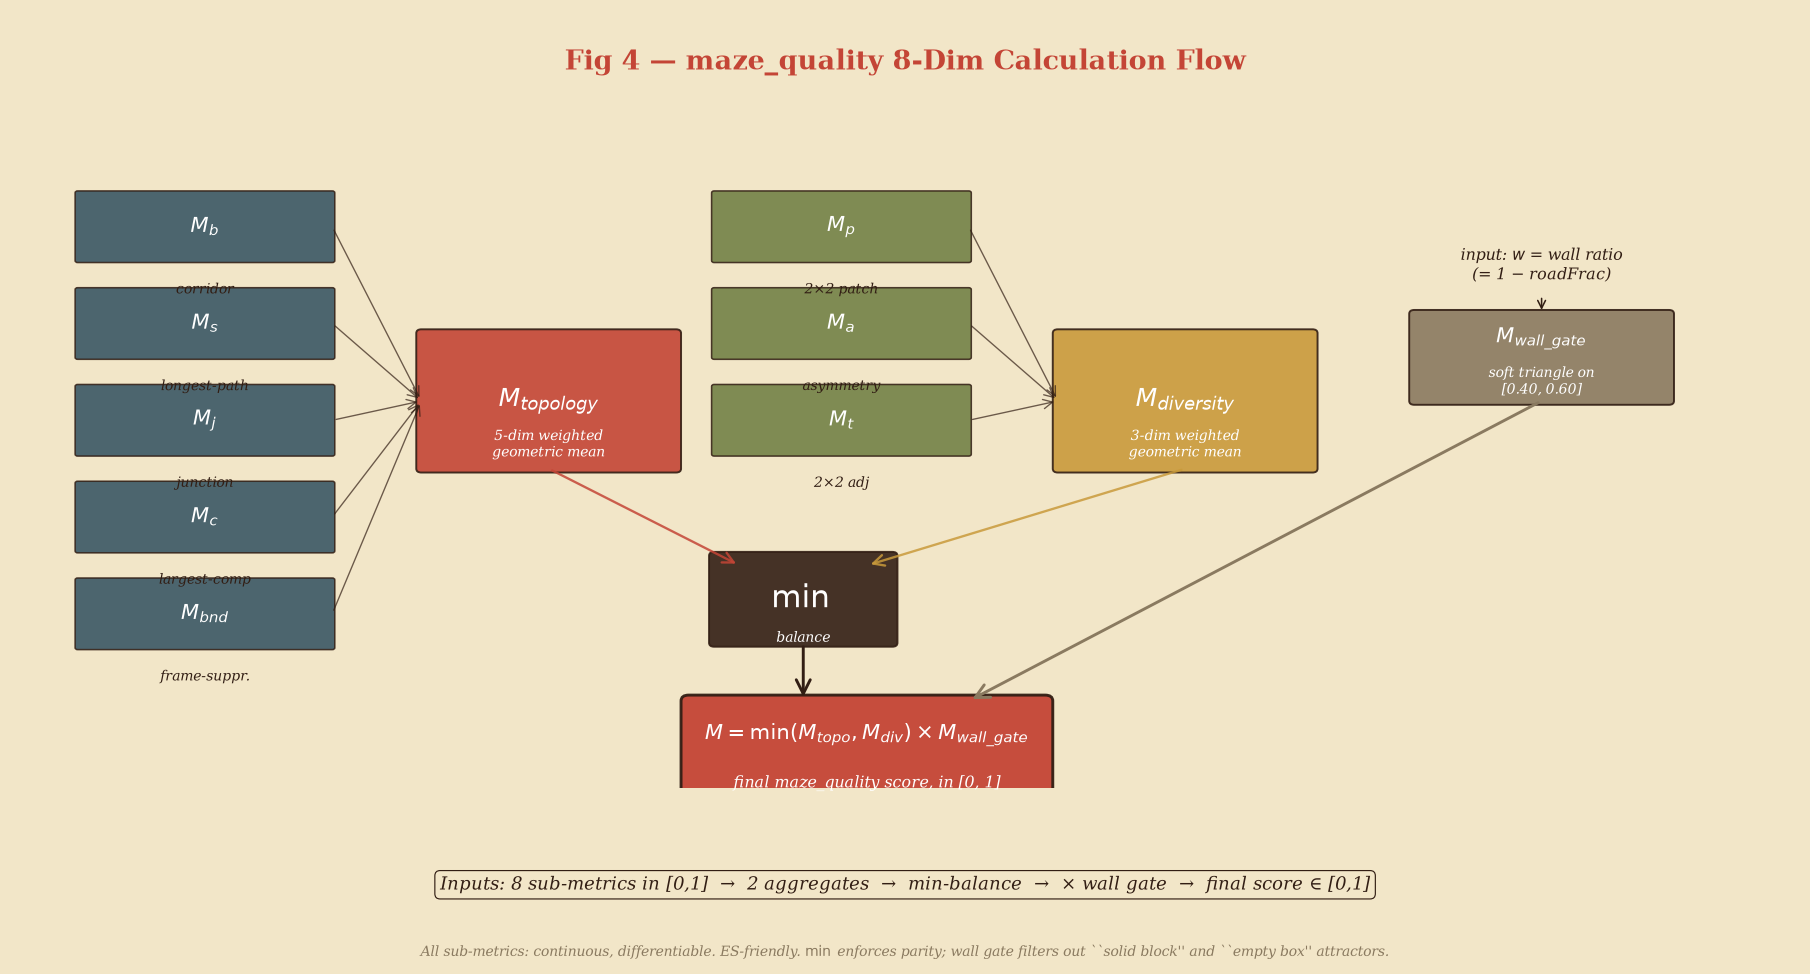
\includegraphics[width=0.96\linewidth]{../figures/v2/fig_mq_calculation_v3.png}
\caption{\textbf{maze\_quality 计算流程。}
8 个连续可微子度量 (左 5 拓扑 + 右 3 多样性) 分别做加权几何聚合得到
$M_{\text{topology}}$ (红) 与 $M_{\text{diversity}}$ (黄);
两侧 $\min$-平衡后乘以 $[0.40, 0.60]$ 上的三角门控
$M_{\text{wall\_gate}}$ (棕, 峰值 1), 得到 final score $\in [0,1]$。
所有算子连续可微, ES 可学; $\min$ 强制 ``topology 与 diversity 同步提升''。}
\label{fig:mq-calc}
\end{figure}

\subsection{15-pattern 对照基准}

$maze\_quality$ 的判别能力用 15 个测试图案做基准评估: 6 个真迷宫生成器 (DFS, Kruskal, Prim, Growing Tree, Sidewinder, Binary Tree) + 9 个几何反例 (Spiral, Fractal Tree, Horizontal Stripes, Random Noise 50\%, Random Noise 30\%, Checkerboard, Diagonal Stripes, Concentric Rings, Honeycomb)。所有图案按 $31 \times 31$ 网格存放于 \texttt{paper/data/\_grids.json}, 分数从 \texttt{paper/data/sweep\_summary.json::15pattern.per\_pattern} 读取并由 \texttt{paper/data/\_eval\_15patterns.mjs} 用真实源码重算交叉验证 (15/15 数值精确匹配, 详见附录 B)。

图~\ref{fig:15pat-mq} 给出 15 张图案的 maze\_quality 分数, 图~\ref{fig:15pat-bellot} 给出 Bellot 2021 $F$ 分数作为对照基线。同一批 15 张图案在两图中的位置严格对应 (5x3 网格, 前 2 行 6 个 TRUE, 后 3 行 9 个 PSEUDO)。

\begin{figure}[H]
\centering
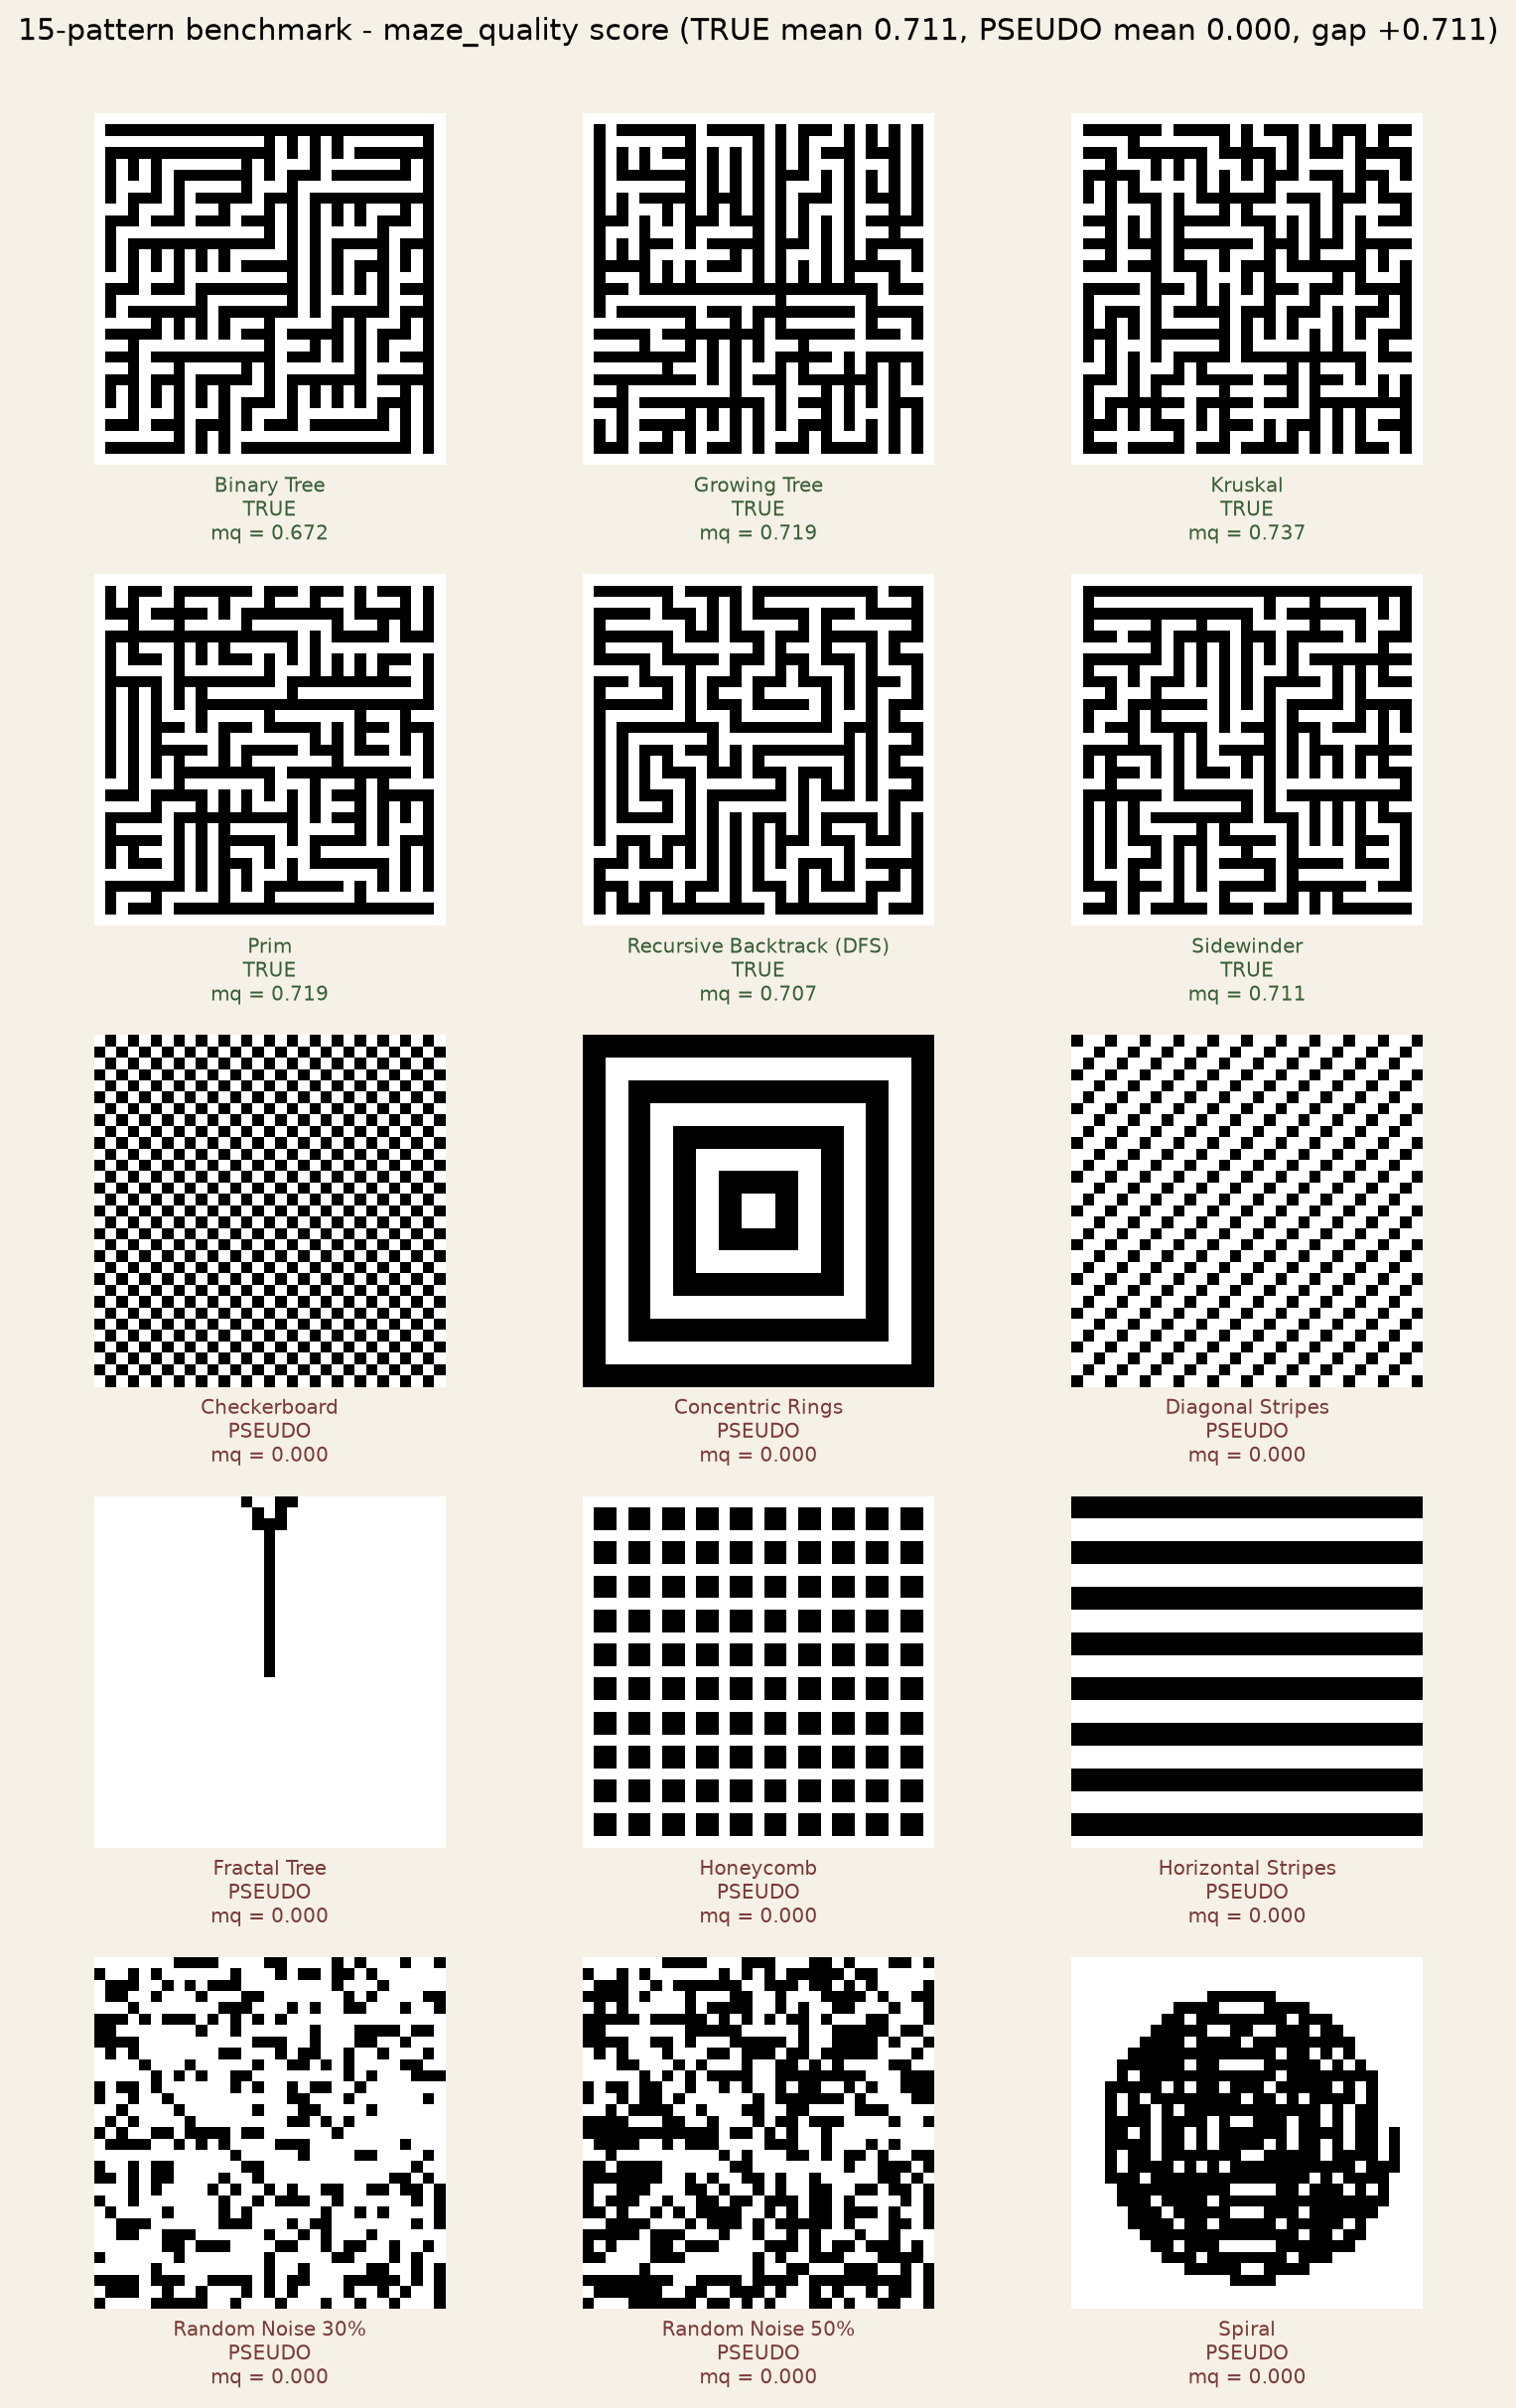
\includegraphics[width=0.78\linewidth]{../figures/v2/fig_15pat_grid_mq.png}
\caption{\textbf{15-pattern maze\_quality 分数。}
6 个真迷宫生成器全部落在 0.672--0.737, 均值 0.711;
9 个伪迷宫全部 0.000。间隔 +0.711, 误判 0/9 (阈值 0.5)。}
\label{fig:15pat-mq}
\end{figure}

\begin{figure}[H]
\centering
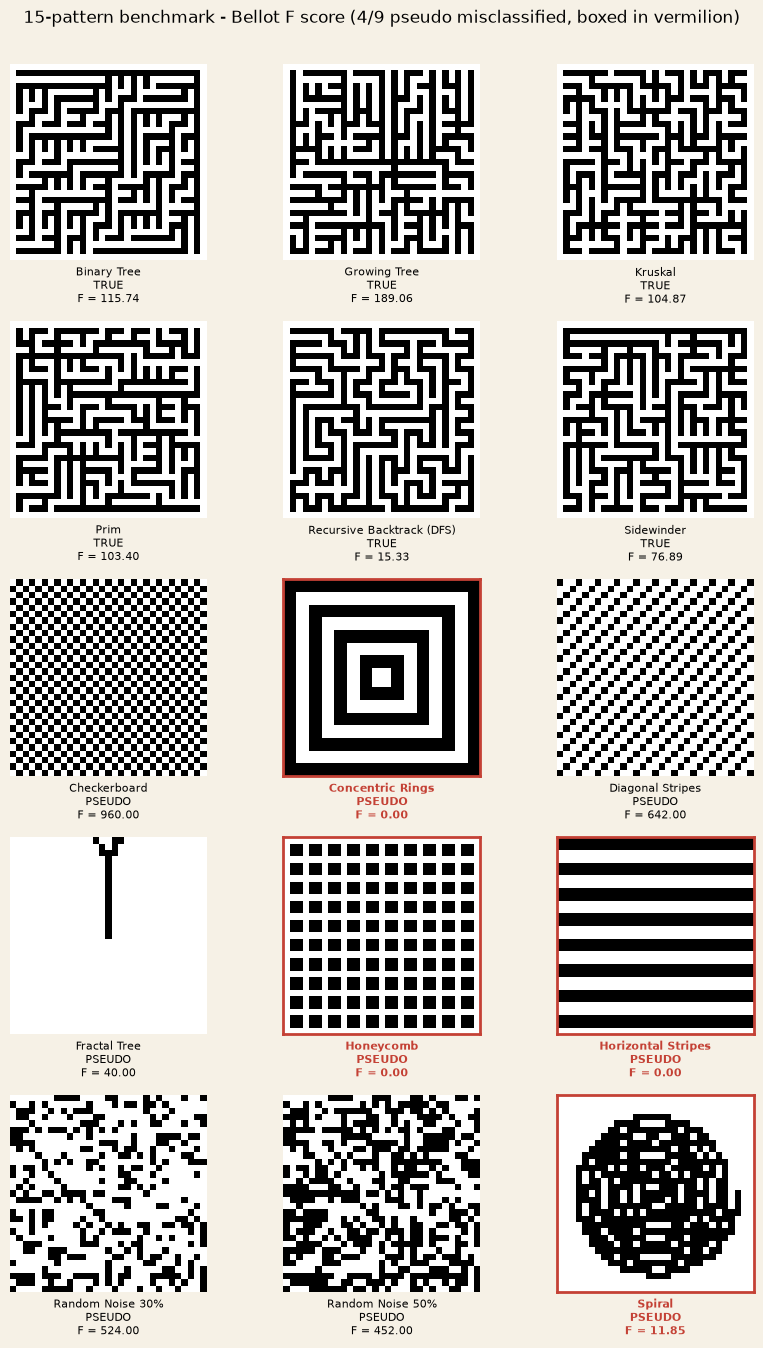
\includegraphics[width=0.78\linewidth]{../figures/v2/fig_15pat_grid_bellot.png}
\caption{\textbf{15-pattern Bellot $F$ 分数 (同一批 15 张图案)。}
真迷宫均值 $F = 100.88$, 伪迷宫均值 $F = 292.21$, 方向反转 (值越小越 ``像迷宫''), 间隔 $-191.32$。
9 个伪迷宫中有 \textbf{4 个} (红框: Spiral $F = 11.85$, Horizontal Stripes / Concentric Rings / Honeycomb $F = 0$)
的 $F$ 值低于真迷宫最低值 ($F = 15.33$, Recursive Backtrack),
即 Bellot $F$ 把它们判为 ``比 DFS 更像迷宫''。}
\label{fig:15pat-bellot}
\end{figure}

两图对比直观给出 $maze\_quality$ 的设计动机: 图~\ref{fig:15pat-bellot} 中 4 个红框图案都是规则几何形态 (条纹, 环, 蜂巢, 螺旋), 全部满足 ``少死端墙 + 长直径'' 的 Bellot $F$ 奖励条件; 而 $M_s$ 在 $L_{\max}/N > 0.5$ 时单调降至 0, $M_j$ 在 $r_j$ 远离 0.10 时呈高斯衰减, 二者在设计目标上显式拒收这类反例。

\subsection{maze\_quality 与 Bellot $F$ 的方向反转}

Bellot 2021 $F$ 报告 ``真迷宫值小, 伪迷宫值大'' \cite{bellot2021}, 与 $maze\_quality$ 的 ``真迷宫值大, 伪迷宫值小'' 方向相反。这个方向反转不是数值巧合, 而是公式定义决定的:
\begin{itemize}[leftmargin=*, itemsep=0pt, topsep=0pt]
  \item $F = \nu / \delta$, 其中 $\nu$ 是 ``非显著墙'' (死端邻接类) 的计数, $\delta$ 是 twistiness proxy。真迷宫 $\delta$ 大 (走廊长程连通) 而 $\nu$ 相对小, 所以 $F$ 小; 伪迷宫 $\delta$ 小 (短路径或几何重复) 而 $\nu$ 相对大, 所以 $F$ 大。
  \item $maze\_quality$ 是几何度量, 越高越像迷宫; $F$ 是 ``像迷宫程度 / twistiness'' 的比值, 越低越像迷宫。
\end{itemize}

4/9 误判的几何机制: Spiral $F = 11.85$ 低于 DFS $F = 15.33$, 因为 Spiral 的 $\nu = 10$ (几乎所有死端墙都相邻) 比 DFS 的 $\nu = 114$ 小, 分子更小导致 $F$ 更小。3 个 $F = 0$ 的图案 (Horizontal Stripes / Concentric Rings / Honeycomb) 因 $\nu = 0$ 导致 $F = 0$, 被 Bellot $F$ 判为 ``最像迷宫''。

$maze\_quality$ 的 $M_s$ 显式惩罚单路径占比过高 ($L_{\max}/N > 0.5$ 时单调降至 0), $M_j$ 显式奖励分叉比例 $\approx 0.10$, 二者共同拒收 Spiral --- 这是设计目标驱动的结果, 不是巧合。
